%*******************************************
\section{Evaluation}
%*******************************************
\label{s:evaluation}
 As a final step the app we have designed and implemented needs to be evaluated which is the goal of this chapter.
 The app will be evaluated with the aid of a user study.
 After introducing our study design, we will state our hypotheses and explain how we are going to measure our statements.
 Finally, we will analyze our results and state our conclusion.


%===========================================
\subsection{Participant Recruitment}
%===========================================
\label{s:participant_recruitment}
This section deals with the participant recruitment for the study.
In order to motivate users to attend our user study a 20\euro Amazon gift was raffled among 4 users.
To reach potential participants we proceeded as follows:

\begin{description}[leftmargin=0cm]
\item[Flyer]  We prepared a flyer with the most important information. 
In this flyer we told the user that a learning app about Internet security in general will be tested. 
We did not mention the specific topic of phishing because we did not want potential participants to read up about it in advance.
One might question our approach of not telling the user what exactly the study is about.
However, we do not consider this an issue since the user was told about the exact topic at the beginning of the study.
Copies of this flyer were hung on blackboards of student dorms and some other buildings at the university.
\item[E-Mail to Professors] We additionally distributed the flyer to a number of professors in our university and asked them to forward it to their students and/or teaching stuff.
We did not forward the flyer to computer science professors or the like since their students and stuff most likely does not match our target group.
\item[Online Social Networks] We contacted our friends in online social networks and asked them to ask friends whether they would be willing to participate in our user study.
Additionally, we posted the flyer in university groups of online social networks with the hope some people might be interested in participating.
\item[Further Networks] Finally, we called friends we could not reach via online social networks and asked them if they knew anybody who would participate.
Also, we tried to approach random people at the university, however this was rather unsuccessful. 
\end{description}

In \autoref{s:participant_recruitment} copies of our e-mails to the professors and of our flyer can be consulted.
Note that we had to split the user study into groups of 4 participants each due to the lack of available smartphones.
Moreover, our flyer originally said that the best participant of each group would win the gift certificate.
However, we recognized that the winning chance might not be equal for every participant, for example, due to varying expertise or other possible technical problems, such as app crashes.
For this reason we asked the participants at the beginnig of each study whether it was okay for them to raffle the gift certificate instead.
Here again it is ethically questionable to award only one of the participants with a gift certificate while others might come away empty-handed.
To address this problem we decided to offer cookies and other kinds of sweets.
Additionally, the participant who performed best was awarded with a ``Golden Anti-Phish Certificate'', all other participants received a ``Silver Anti-Phish Certificate''.

%===========================================
\subsection{Study Design}
%===========================================
For our user study we chose a within-subject design, i.e. a ``before and after app'' study with the same group of people.
The advantages of this design can be summarized as follows:
Within-subject deals better with variability associated with individual differences compared to between-group design, where different groups would be considered who do and do not play the app.
Furthermore, if we had decided for the between-group design we would have needed twice as many participants which we would have not been able to recruit.
A major drawback of the withing-subject design, however, is the learning effect.
We are not able to clearly distinguish whether a behavior change after playing the app is a result of the app intervention or whether the paricipants just have overthought their decisions on questions they had replied to before.
Yet, our results showed that this learning effect can more or less be ignored (cf. \autoref{s:hypanalysis}).
\autoref{fig:study_structure} illustrates the structure of our study, which we explain in the following: 
\begin{enumerate}
	\item \textit{Informed Consent} Before starting the user study the participants have to sign an informed consent.
This form briefly explains what the study is about and clarifies that the participant is not obliged to finish the study.
If the user terminates the study before finishing it, however, he cannot participate in the gift certificate raffle.
Optionally, the user can agree with the anonymous publication of the:
	\begin{enumerate}
		\item transcriptions of the study (recordings will be deleted after the study)
		\item filled out surveys
	\end{enumerate}

	\item \textit{General-Survey Before} At the beginning the participants have to fill out a general survey, where they have to judge their own knowledge on the topic of Internet security in general.
 For instance, they are asked whether it is easy for them to distinguish legitimate e-mails and websites from fake ones.

	\item \textit{Website-Survery Before} In this part of the user study the participants gets a list of screenshots of websites.
 The screenshots had been taken with the standard browser of an Android tablet.
 In total, the user is shown 16 screenshots, with 8 phishing and 8 valid URLs.
 The user has to decide whether he would enter confidential data on the shown website.
 Additionally, he has to encircle the part of the screenshot which was the primary reason for his decision.
 Then, the user has to indicate how sure he was about his answers on a Likert scale.
 Finally, the user is asked whether he knows the vendor of the website and whether he has a account there.

	\item \textit{Play App} After the ``Website-Survey Before'' the users get the smartphones in order to play the app.
 To save time, we skipped the introduction 2 part (access address bar) for the user study.
 The user has half an hour to play the app.
 After half an hour they are asked to put the smartphones aside.
 Then, we collect the smartphones and note the reached points in each level.

	\item \textit{Website-Survery After} After playing the app, the participants get a second website-survey.
 In this, all examples of the previous survey are included.
 Moreover, it contains 8 further website screenshots of which 4 have phishing and the remaining 4 have valid URLs.

	\item \textit{General-Survey After} Here, the participants are asked to fill out a form with questions to their demographics.
 This form does also contain questions related to the SUS and some other questions regarding their impression of the app.
	
	\item \textit{Certificates} At this point the official study is finished.
We thank the users for their participation and award a ``Golden Anti-Phish Certicate'' to the best participant of the current group.
All other users receieve a ``Silver Anti-Phish Certificate''.
Next, the gift certificate is raffled.

	\item \textit{Debrief} Finally, an optional debrief follows, where the users can ask questions or provide their remarks in person.

\end{enumerate}



\begin{figure}[hHtbp]
\centering
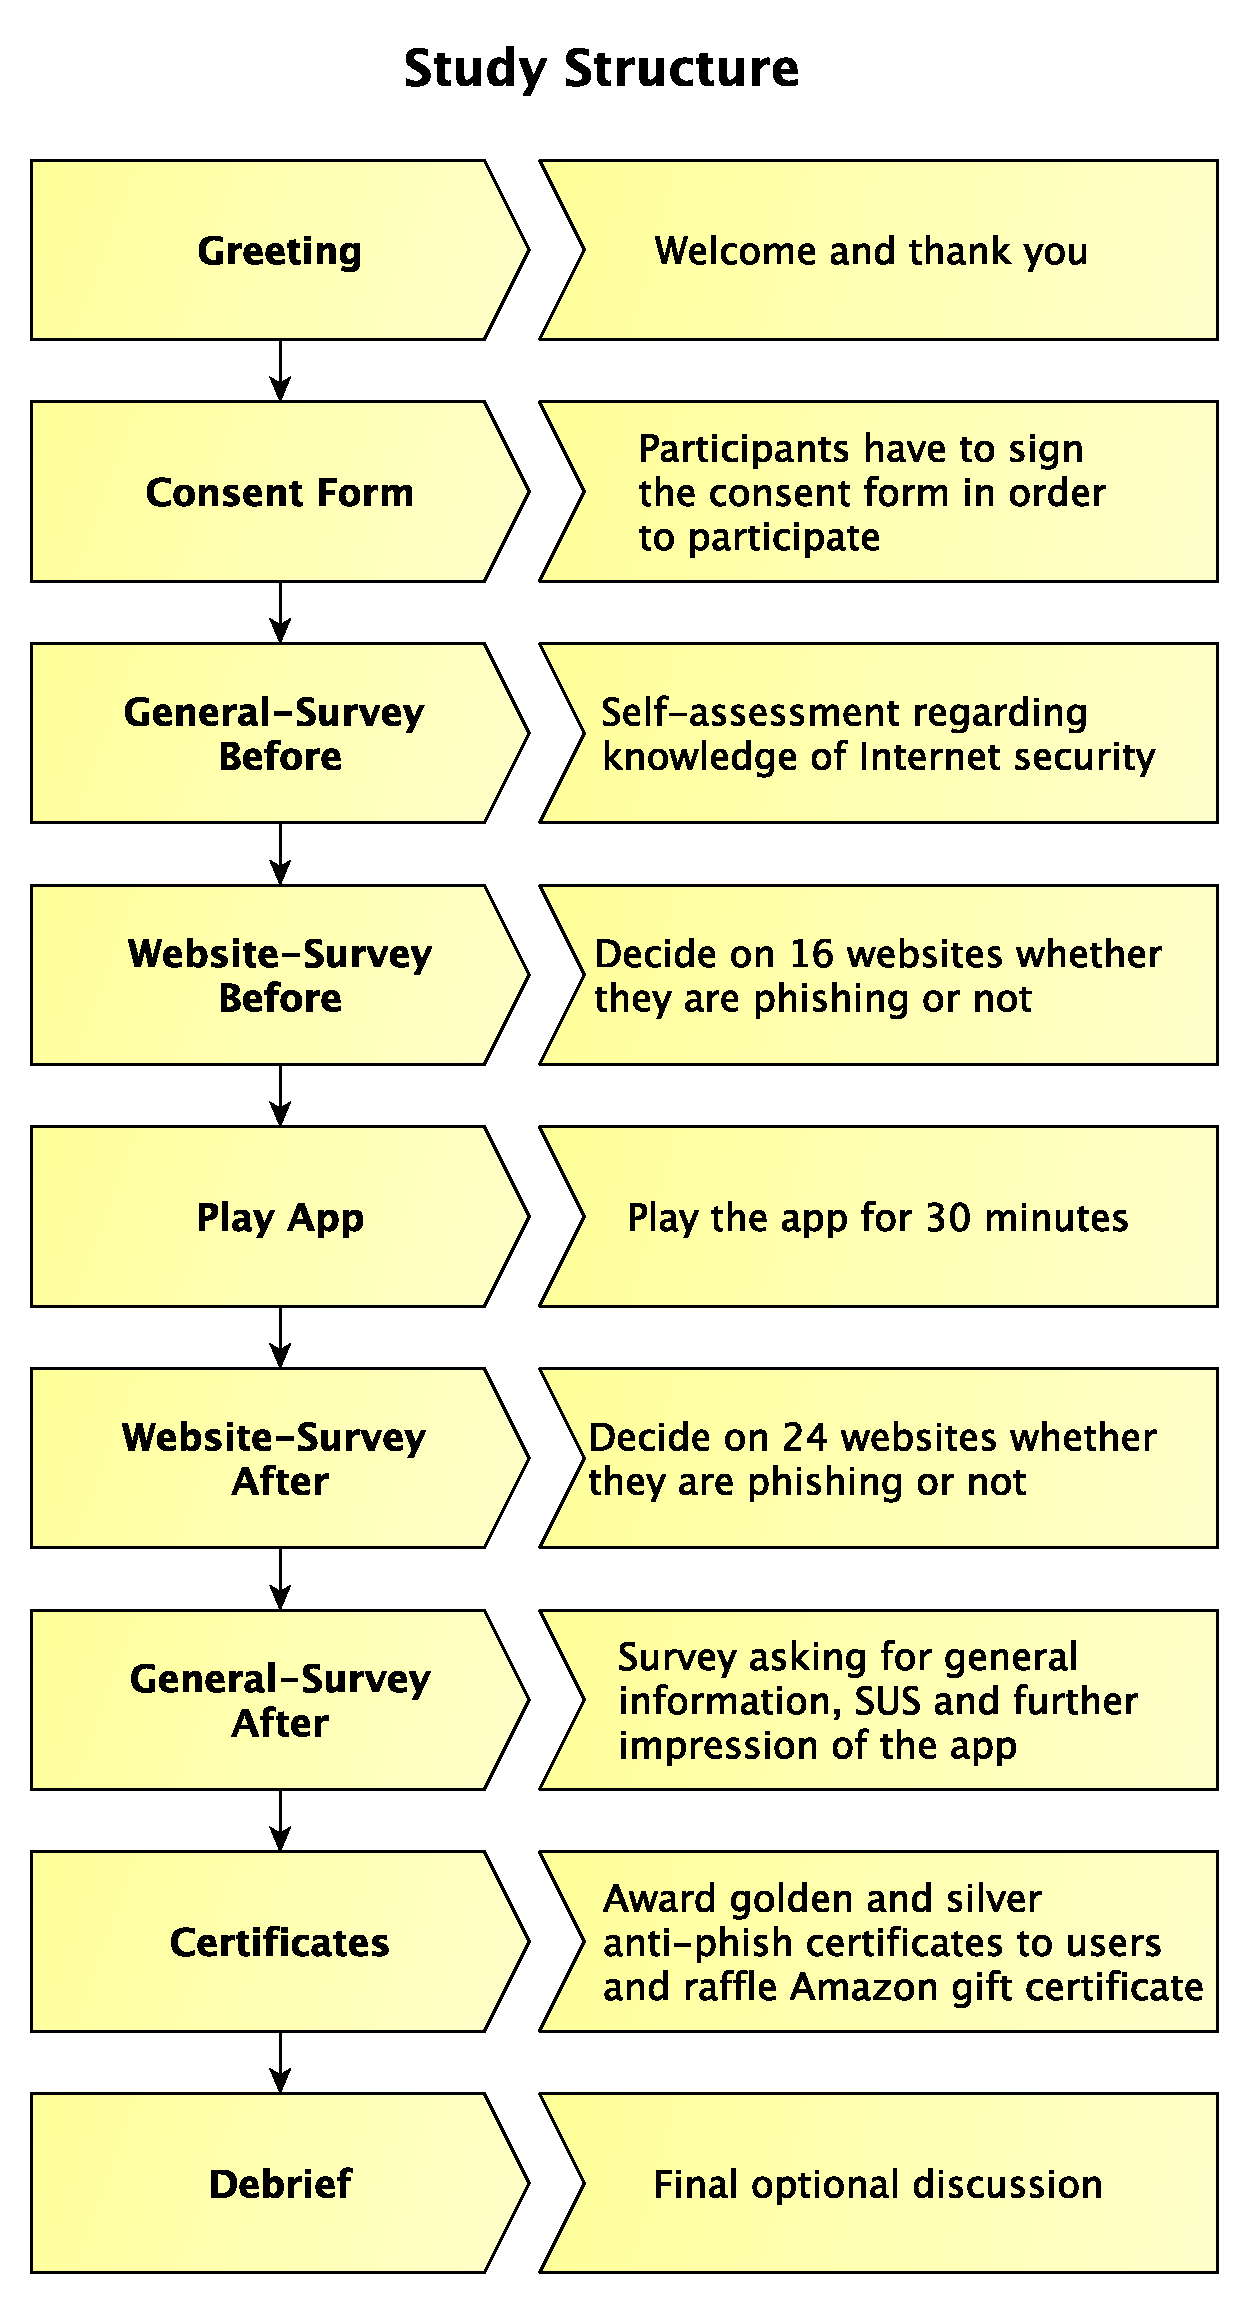
\includegraphics[height=0.9\textwidth]{study_structure.pdf}%
\caption{Our study structure}%
\label{fig:study_structure}%
\end{figure}

\subsubsection{Limitations}
We have decided to conduct a study which compares the users' performance before and after playing our educational app.
Our study design has some limitations we were not able to address for several reasons.
This section discusses these limitations.

\begin{description}[leftmargin=0cm]
	\item[Behavior Change] In our study the participants were not in their usual environment. 
	Therefore, they likely behaved differently during our study.
	An alternative approach was to distribute the app to several participants and ask them to play it remotely.
	However, this has two major downsides: First, the user would have been remote and thus we would have less control.
	Second, testing the before and after app skills would have been difficult to realize.
	\item[Increased Attention] At the beginning of the study the participants were told that the study dealt with phishing.
	Additionally, for the website-survey before and after they were explicitly asked to indicate whether the websites were phishing or not.
	That is to say, the user automatically increased his attention towards answering this question.
	In fact, this is not close to reality.
	Designing an in situ study, where the participant would have been in their usual environment and would have not known about their participation, was not considered for time reasons and, most importantly, because such a design is ethically and legally questionable. 
	For these reasons the post influence of the app could also not be tested.
	\item[Retention] Our study design focuses on the present.
	For time reasons we did not have the possibility to repeat the ``after app'' scenario after some time has passed.
	Consequently, retention is an aspect which is not considered by our study.
	\item[Bias] For the recruitment we endeavored to ensure that our participants are not close friends of ours. 
	We rather seeked for friends of friends or even completely unknown persons by, for instance, hanging out our flyers and contacting several professors~(cf. \autoref{s:participant_recruitment}).
	In order to further avoid biases the study should have been conducted by other persons than us.
	The fact that the participants were in contact with us, the app designers and developers, during the study might have caused a bias.
	Yet, we believe that the potential bias is negligible since the participants' feedback was not outstandingly good.
	Their feedback was generally positive, but some of the participants also criticized several aspects of the app~(cf. \autoref{s:further_exploration}).
\end{description}

Despite the limitations of our study we believe that we could get a good insight into the effectiveness of our app.
In the succeeding sections we will elaborate on the hypotheses we constructed in the previos section and analyze them.
%===========================================
\subsection{Hypotheses}
%===========================================
In order to evaluate the effectiveness and usability of our app we have formulated below mentioned hypotheses and measurements.
As aforementioned, users are asked to encircle the area of the screenshot which was the primary reason for their decision.
The coding of these markings, which are relevant for our measurement, can be consulted in \autoref{s:markings}.

\begin{enumerate}
	\item \textit{Hypothesis 1 - Mistakes} After playing the app, the users make significantly less mistakes when deciding whether a website is a phish or not.\newline
	Measurement: Correctly identified websites in ``Website-Survery After'' (phish or no phish) $>>$ correctly identified websites in ``Website-Survery Before''
	\item \textit{Hypothesis 2 - URL Based Decision} After playing the app, the users base their primary decision on whether a website is a phishing website or not significantly more often based on the URL compared to before playing the app.\newline
	Measurement: Number of URL markings in ``Website-Survery After'' $>>$ number of URL markings in ``Website-Survery Before''
	\item \textit{Hypothesis 3 - URL Comprehension} After playing the app the user understands the importance of the domain of a URL as the only criteria to detect phishing websites\newline
Measurement: Number of marked URL domains in ``Website-Survery After''  $>>$ number of marked URL domains in ``Website-Survery Before'' 
	\item \textit{Hypothesis 4 - Good Usability} The app usability is above average. \newline
Measurement: According to~\cite{sus}  a System Usability Scale (SUS) $>$ 68 can be considered above average usability.
\end{enumerate}

%===========================================
\subsection{Coding of Markings}
%===========================================
\label{s:markings}
In the previous section we stated our hypotheses and how we decided to measure them. For Hypothesis 3 it is interesting to specify what marking of what area we consider as separate option.
Here, we provide an overview of our coding for possible markings in the website-surveys.
These codings are relevant for the measurement of our hypothesis 3.

\begin{enumerate}[leftmargin=0cm]
	\item\textit{None} Occasionally, participants did not mark or encircle anything of the screenshot. In our raw data this is coded as none.
	\item\textit{Favicon or Padlock} The marking of a favicon or padlock is trivially coded accordingly.
	\item\textit{Content} If anything else than the URL itself, a part of the URL, a favicon, or a padlock is marked then this is coded as content.
	\item\textit{Scheme} If the scheme or a part of the scheme in a URL is marked, this is coded as scheme.
	\item\textit{Host} Marking the host results in an according coding.
	\item\textit{Domain} In case a participant marks a domain or the substring of a domain this is coded as domain or domain substring accordingly.
For the measurement of hypothesis 3, domain as well as domain substring markings are considered domains.
	\item\textit{URL} All other markings are coded as URL and measured as such.
\end{enumerate}


%===========================================
\subsection{Results and Analysis}
%===========================================
This section presents our results and analyzes them. 
We start with discussing the representativeness of our participants and proceed with illustrating interpretation problems we faced while we assessed the website-surveys.
Therafter, we analyze and present the results of our measurements to our hypotheses and proceed with some further exploration of our results.
Finally, this chapter is closed with our discussion and conclusion.


%.........................................................................................................
\subsubsection{Representativeness}
%.........................................................................................................
\label{s:representativeness}
In general we took care that the people we tried to recruit do not have extensive prior knowledge on this topic.
For example, our flyer asked for non-specialists.
Yet, we were not able to assure beforehand that we would only have non-specialist participants.
In such a case we had to rule them out for our analysis afterwards.
Unlike in our phishing survey (cf. \autoref{s:survey}), where we ruled out electrical engineers or computer scientists in general, we did not generally exclude those from our final user study.
The problem with the phishing survey was that it did not give us enough indication whether a particular participant was too skilled for our target group.
Therefore, we had to imply that computer scientiests and electrical engineers are too skilled for our target group, even if this does not necessarily need to be the case in reality.
In fact, there might be computer scientists or electrical engineers who can learn something from our app.
In the contrary, in our final user study we were able to determine a user's prior knowledge more precisely with the aid of the website-survey before.
Therefore, we did not primarily consider their course of study or field of work, but rather how well they performed in the website-survey before playing the app (cf. \autoref{s:hypanalysis}).
Finally, we made an effort to recruit participants who are not close friends of ours in order to minimize biases.

%.........................................................................................................
\subsubsection{Marking Interpretation}
%.........................................................................................................
\label{s:intprobs}

As aforementioned, the study participants were asked to fill out a website-survery before and after playing our app.
In this survey they had to indicate whether a given screenshot of a website is a phish or not.
Furthermore, they were asked to encircle the area of the screenshot which was the primary reason for their decision.
This section first shows some examples for the marking codes depicted in \autoref{s:markings}.
Afterwards, we illustrate you the challenges we had to face when interpreting the users' markings, as they were not always clear.

\begin{description}[leftmargin=0cm]
	\item[Marking Interpretation Examples] As aforementioned, we categorized the possible markings of users into favicon, padlock, content, scheme, host, domain (substring), and URL in general.
\autoref{fig:content} and \autoref{fig:padlock}, for example, illustrate samples where the content or the padlock of a website was marked.
\autoref{fig:m_domain} and \autoref{fig:m_domain_substring} depict examples where the markings were interpreted as domain and domain substring.
A sample where the host is marked is illustrated in \autoref{fig:m_host}.
And finally, \autoref{fig:m_url_02} shows an example of a marking (subdomain) which is coded as URL in general. 

	\item[Interpretation Problem Examples] While assessing and digitalizing our data we had to face some interpretation problems which we exemplify in the following.
In such cases we had no choice but trying to interpret the samples as objectively as possible.
\autoref{fig:m_content_or_host}, for instance, shows a marking where the circle includes the content (youtube logo) as well as the host. 
For this sample, we decided to code this marking as host.
The next examples in \autoref{fig:m_domain_or_not} shows a marking where a subdomain and the domain is marked. 
When we faced examples like this we decided to code it as domain in case a subdomain is only partially marked, so that there is an indication that the user just did not make his markings clear enough.
If the subdomain is obviously marked intendedly, i.e. clearly inside the circle, this kind of sample is coded as URL.
In this case we see that the subdomain is inside the circle, for this reason we coded this sample as URL.
A sample we came across often is a participant making two markings, even though we explicitly asked to mark only one area.
In these cases we decided as follows: in case a marking is obviously striking due to a thicker circle, for instance, the more emphasized area is chosen for coding.
Should both markings be kind of equal, we joint the markings and decided based on that.
In \autoref{fig:m_url} a participant marked the scheme and the host separately. 
We cannot observe any emphasis on one of the markings.
Therefore, we chose to code this sample as URL.
Finally, there were samples where the user correctly identified a phishing website.
However, instead of marking the domain as reason, what we expected from the participants, some users marked the attacked part instead.
\autoref{fig:m_attack_recognized} illustrates such an example.
In fact, this reason is justified. 
Yet, we had to code such samples as URL since there is no clear way of defining the code for recognizing the attacked part of a URL.
\end{description}

\begin{figure}
\centering
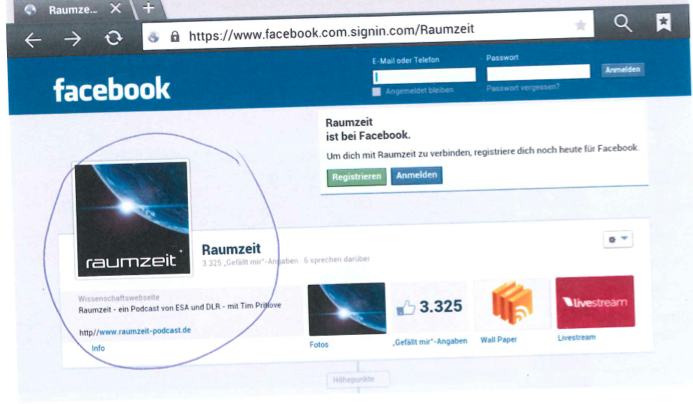
\includegraphics[width=0.8\textwidth]{m_content.png}
\caption{Content marked}
\label{fig:content}
\end{figure}

\begin{figure}
\centering

\includegraphics[width=0.8\textwidth]{m_padlock.png}
\caption{Padlock marked}
\label{fig:padlock}
\end{figure}

\begin{figure}
\centering

\includegraphics[width=0.8\textwidth]{m_domain.png}
\caption{Domain marked}
\label{fig:m_domain}
\end{figure}


\begin{figure}
\centering

\includegraphics[width=0.8\textwidth]{m_domain_substring.png}
\caption{Domain substring marked}
\label{fig:m_domain_substring}
\end{figure}

\begin{figure}
\centering
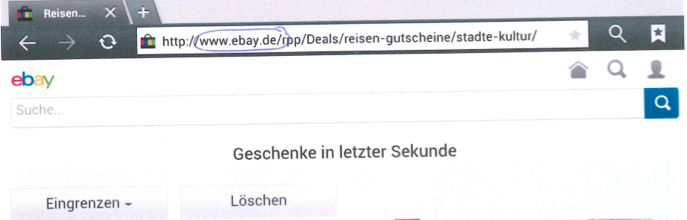
\includegraphics[width=0.8\textwidth]{m_host.png}
\caption{Host marked}
\label{fig:m_host}
\end{figure}

\begin{figure}
\centering
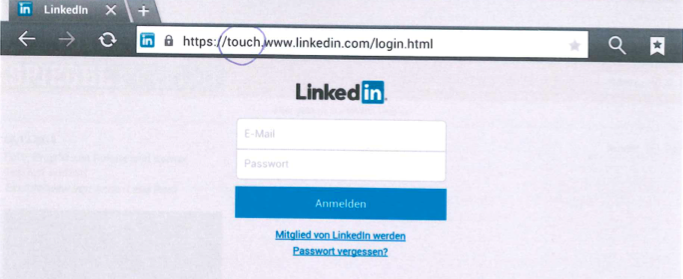
\includegraphics[width=0.8\textwidth]{m_url_02.png}
\caption{Subdomain marked, coded as URL}
\label{fig:m_url_02}
\end{figure}

\begin{figure}
\centering
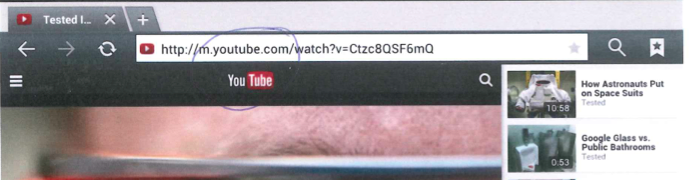
\includegraphics[width=0.8\textwidth]{m_content_or_host.png}
\caption{Host or content marked?}
\label{fig:m_content_or_host}
\end{figure}

\begin{figure}
\centering
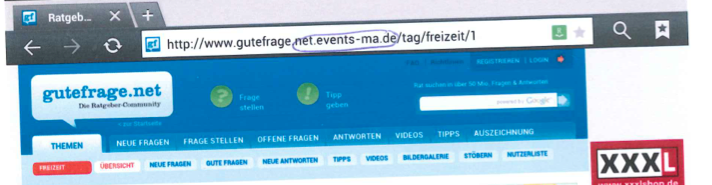
\includegraphics[width=0.8\textwidth]{m_domain_or_not.png}
\caption{Domain or URL marked?}
\label{fig:m_domain_or_not}
\end{figure}

\begin{figure}
\centering

\includegraphics[width=0.8\textwidth]{m_url.png}
\caption{Scheme or host marked?}
\label{fig:m_url}
\end{figure}

\begin{figure}
\centering

\includegraphics[width=0.8\textwidth]{m_attack_recognized.png}
\caption{Attack marked}
\label{fig:m_attack_recognized}
\end{figure}


%.........................................................................................................
\subsubsection{Analysis of Our Hypotheses}
%.........................................................................................................
\label{s:hypanalysis}
In total 19 participants attended our study (one participant did not show up).
As discussed in \autoref{s:representativeness} we did not rule out any participant beforehand.
In fact, wer had to sort out two part two users for the results and analyses of our study:

\begin{enumerate}
	\item\textit{Outlier} \autoref{fig:outlier} depicts the performance of our participants.
	It illustrates how many URLs were correctly identified by how many users.
	Evidently, there is an outlier among our participants. 
	One user gave 15 correct answers to 16 questions.
	Thich means that he has too much prior knowledge on this topic and thus does not match our target audience.
	Therefore, this participant is not considered for our further elaborations.
	\item\textit{Seriousness} Another participant obviously did not engage himself to play our app.
	During the 30 minutes of playing the app the user managed to complete the awareness part and level 1 (identify domain) only.
	More importantly, we saw the user playing around with the Samsung device instead.
	Since this user did not seem to take our study and app seriously we decided to sort him out for further considerations.
\end{enumerate}

\begin{figure}
\centering
\subfigure[Before]{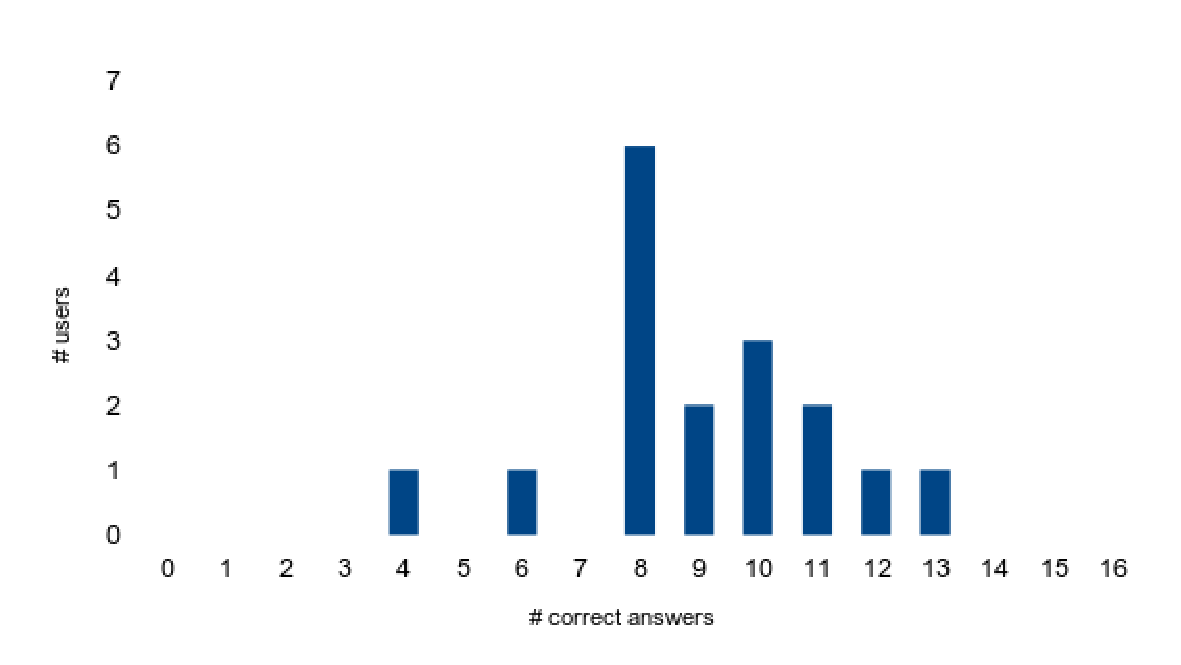
\includegraphics[width=0.45\textwidth]{hyp1b.pdf}}
\subfigure[After (all URLs)]{\label{fig:hyp1resultsaall}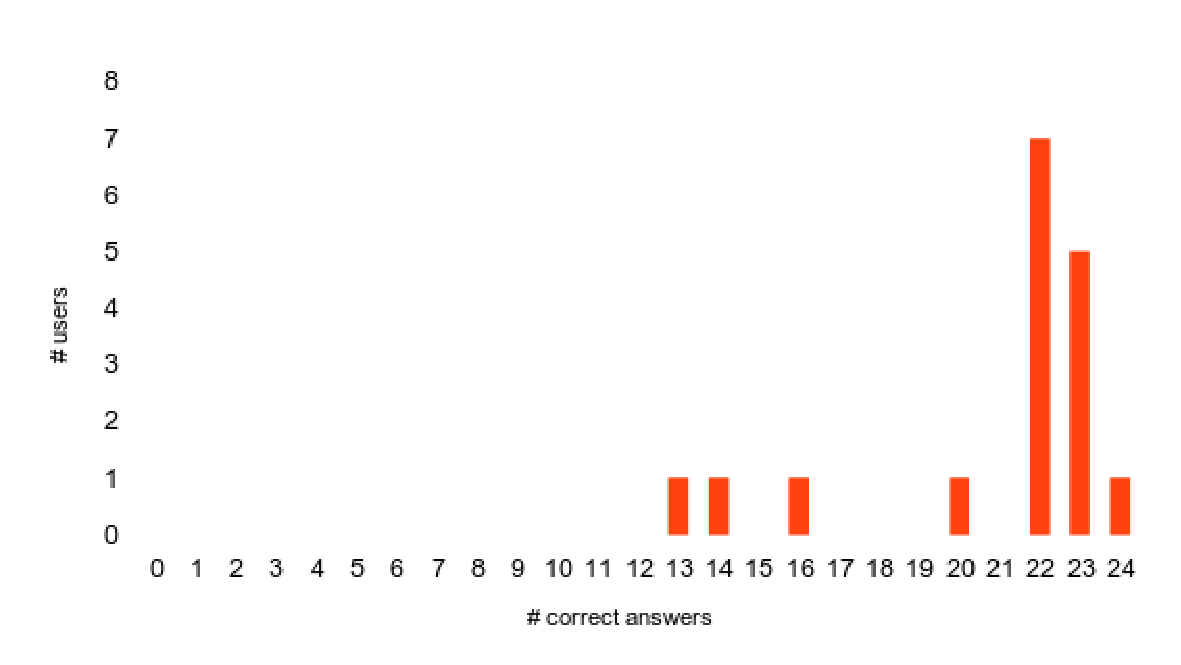
\includegraphics[width=0.45\textwidth]{hyp1a.pdf}}
\subfigure[After (New URLs)]{\label{fig:hyp1resultsanew}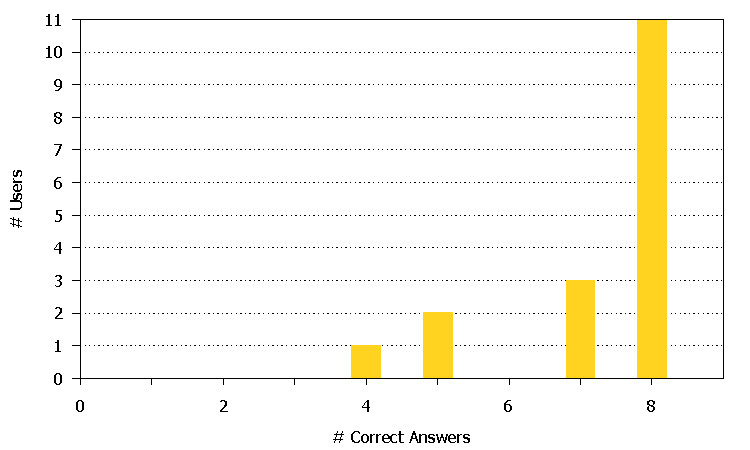
\includegraphics[width=0.45\textwidth]{hyp1anew.pdf}}
\subfigure[After (Repeated URLs)]{\label{fig:hyp1resultsarepeat}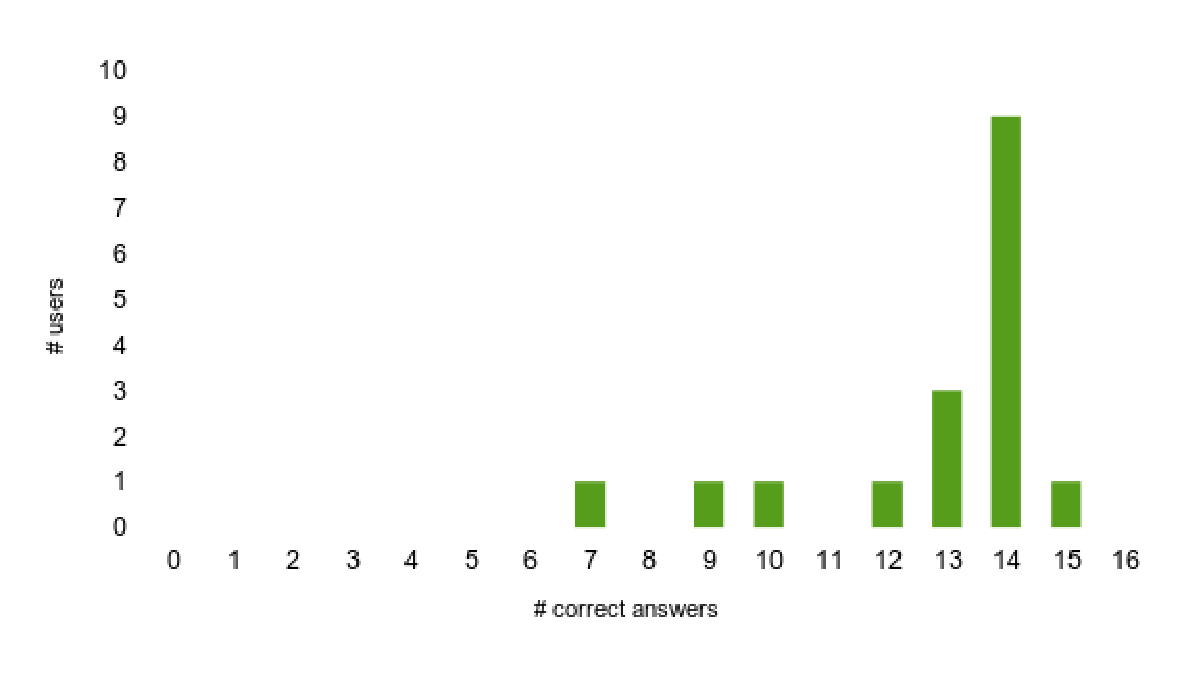
\includegraphics[width=0.45\textwidth]{hyp1arepeat.pdf}}
\caption{Correct Answers}
\label{fig:hyp1results}
\end{figure}

\begin{figure}
\centering
\subfigure[Before]{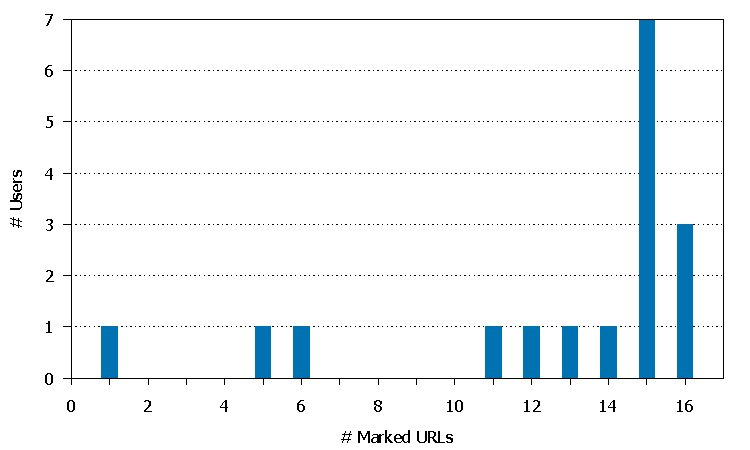
\includegraphics[width=0.45\textwidth]{hyp2b.pdf}}
\subfigure[After]{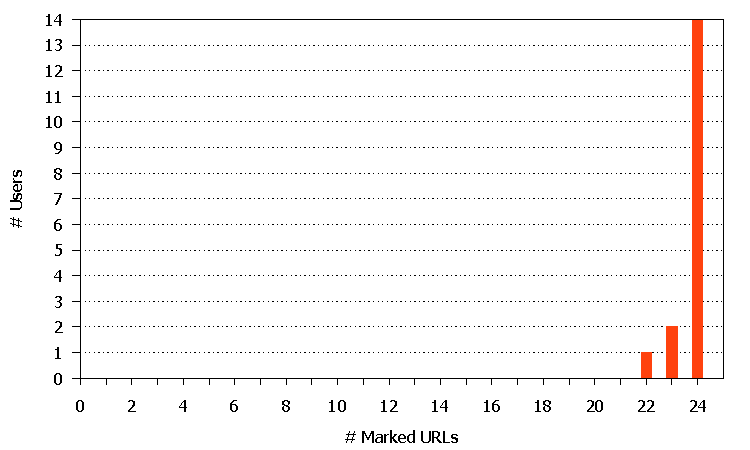
\includegraphics[width=0.45\textwidth]{hyp2a.pdf}}
\caption{URL marked}
\label{fig:hyp2results}
\end{figure}

\begin{figure}
\centering
\subfigure[Before]{\label{fig:domain_before}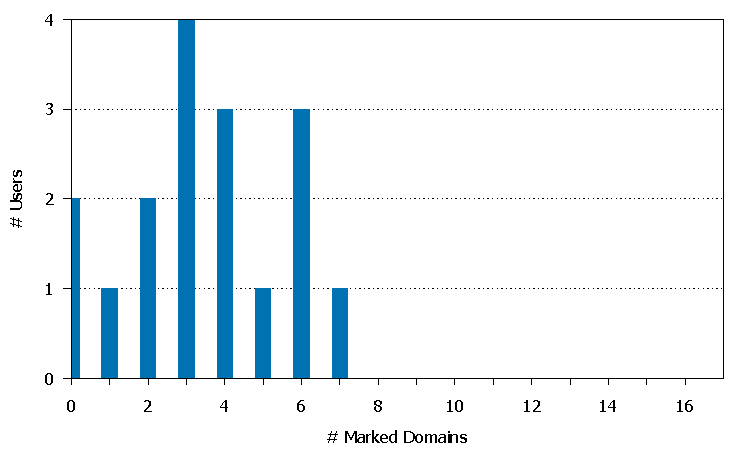
\includegraphics[width=0.45\textwidth]{hyp3b.pdf}}
\subfigure[After]{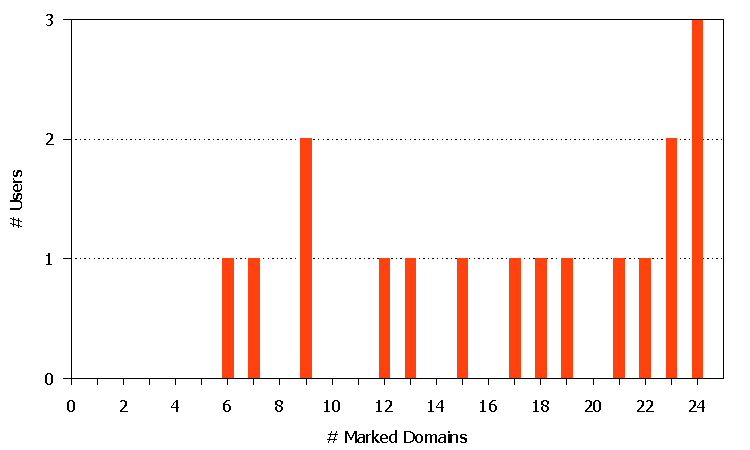
\includegraphics[width=0.45\textwidth]{hyp3a.pdf}}
\caption{Domain marked}
\label{fig:hyp3results}
\end{figure}

\begin{description}[leftmargin=0cm]
\item[Hypothesis 1]
\autoref{fig:hyp1results} shows the results of our study according to hypothesis 1. One can clearly see that the majority of the users identified more URLs correctly after using the app than before. While most participants correctly identified 8 out of 16, i.e. 50\%, websites before they played the app, the majority gave correct answers to 22 out of 24 websites afterwards, i.e. 91.67\%. One could argue that this increase is based on the fact that the examples are mainly the same in the website-survey after, i.e. the reason for their better performance is based on learning effects. \autoref{fig:hyp1resultsanew} however shows that the user also gave correct answers to most of the new URLs. Therefore, we assume the learning effects are negligible.
In order to affirm our hypothesis we decided to apply the onesided Wilcoxon signed-rank test~\cite{wilcoxon1945individual} with our 16 samples from the website-survey before and the same 16 samples from the website-survey after.
Since we consider the learning effects negligible, we do not apply an alternative test against the 24 after URLs.
Our null hypothesis is $H_{0} = x_{1} >= x_{2}$ and the alternative hypothesis $H_{1}: x_{1} < x_{2}$, where x$_{1}$ represents the number of URLs which were correctly answered before playing the app and x$_{2}$ represents the number of URLs which were correctly identified after playing the app.
We computed the positive and negative rank-sums of $W_{+} = 141.5$ and $W_{-} = 11.5$.
The test statistic $w$ is the minimum of $W_{+}$ and $W_{-}$, hence $w = 11.5$.
As we chose $\alpha = 5\%$ as significance level and had 17 participants this results in a critical value of $41$.
As our test value $w = 11.5 < 41$ the nullhypothesis can be rejected and thus the alternative $H_{1}$ is accepted.
Consequently, after playing the app the participants gave more correct answers than before.
We are aware that we cannot fully rule out the possibility that there might be kind of learning effect.
Yet, we are confident that these results cannot entirely be reduced to learning effects.
Therefore, we believe that our app helped users to make improved decisions about the legitimacy of URLs.
\item[Hypothesis 2]
\autoref{fig:hyp2results} shows how many users marked the URL as their main source of decision.
Most of the users already based most of their decisions on the URL before.
Occasionally users marked the content or the padlock.
However only 3 Users (17.65\%) always marked the URL.
Afterwards we see that most users (82.35\%) always based the decision on the URL and only 3 Users made on or two mistakes.
Therefore we think that our app emphasized their believe in basing their decision on the URL.
We however think it is important to tell the user this to get uncertain or unknowing users to the same level as most of our participants.
Also our app empathizes the importance of the URL by putting the main focus on it.
We have decided against doing statistical test on this hypothesis.
We believe it will most likely be rejected because the change from before to after is not very high.
\item[Hypothesis 3]
There is a general problem with one question in the websites-surveys.
In the before survey we were not able to clearly ask the user to mark the domain when it was the base of his decision because we would have then primed them towards looking at the URL or even at the domain.
This would have influenced the results of hypothesis 2.
Since we could not formulate this question clearly, a user might have marked the whole URL even if his decision was based only on a small part (e.g. the domain) of the URL.
Consequently, we were not able to clearly identify what the users' main source of decision was in the before survey.
We were aware of this problem beforehand but saw no other option than formulating the question in such an open form.
Afterwards, the user knew that they were expected to mark the domain.
This can be interpreted as a change of question even if the literal question did not change.
Therefore, we cannot apply any statistical tests on this hypothesis.
Yet, we want to have a look at the results.
None of the users marked the domain in most cases beforehand, in particular, 7 domains out of 16 URLs where marked at most by only one user, cf. \autoref{fig:domain_before}.
\begin{figure}
\centering
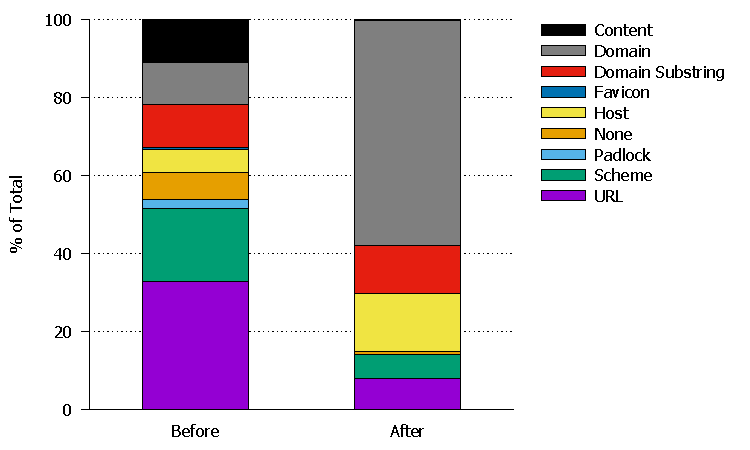
\includegraphics[width=0.45\textwidth]{markings.pdf}
\caption{Marked parts of the screenshot before and after}
\label{fig:markings}
\end{figure}

\begin{figure}
\centering
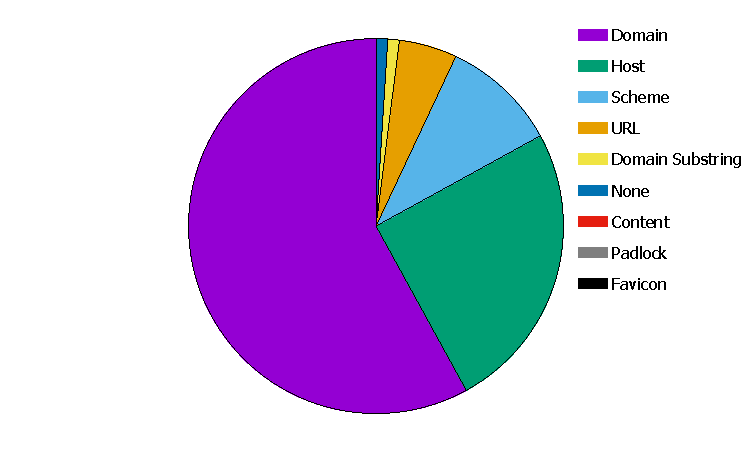
\includegraphics[width=0.45\textwidth]{legitimate_markings_after.pdf}
\caption{Marked URL parts of legitimate URLs}
\label{fig:legitimate_markings_after}
\end{figure}
\autoref{fig:markings} shows the distribution of the marked areas before and after playing our app. Obviously, afterwards most of the users marked the domain. However we are not able to compare that to the before values because of the changed question.
Another interesting observation is that quite a number of participants marked the complete host (instead of the domain) in case of legitimate URLs, cf.~\autoref{fig:legitimate_markings_after}. One explanation for this might be that we did not ask the user to mark the domain of legitimate URLs except in level 1.
\item[Hypothesis 4]
According to the answers that the users gave in the After survey SUS section (\autoref{s:after_survey}) we calculated a SUS of 83.1. This is above 68 which means that we can consider our app above average usable.
\end{description}

%.........................................................................................................
\subsubsection{Further Exploration}
%.........................................................................................................
\label{s:further_exploration}
Besides the results of our hypotheses the study yielded some further interesting outcomes.
This section further explores these results.


\begin{description}[leftmargin=0cm]
	\item[Correct and Reasoned Answers] Hypothesis 1 only refers to giving a correct answer to the question whether a website is a phish or not.
	Our results show that users did not only give more correct answers after playing the app.
	In addition to their correct answer they reasoned their answer appriopriately (i.e. marked the domain).
	In the website-survey before 37.5\% of the URLs were answered and reasoned correctly.
	After playing the app 75\% of the URLs were correctly identified and reasoned. 
	Note, that reasoned means by our definition that the domain was marked in addition to giving a correct answer.
	However, a reasoning must not always rely on the domain itself. 
	As discussed in \autoref{s:hypanalysis}, for example, there were numerous participants who often marked the host of legitimate URLs.
	This is a correct reasoning for their decision, however by our definition it was not considered as such.
	Also, there were plenty of users who detected a phish and marked the attacked part instead (cf. \autoref{fig:m_attack_recognized}).
	By our definition this was also not accepted as correct reasoning.
	Hence, if we had expanded our definition of reasoning even more users would have correctly reasoned their decisions.
	However, there is the question whether expanding the accepted answers might also result in an increase of the correct answers and markings in the before survey.
	\item[User Opinions to App] A part of our surveys tried to understand the users' opinions to our app.
	Section 3 of our survey-after (cf.~\autoref{s:after_survey}) contains the statements which the users had to assess with the aid of a Likert scale.
	Our worst score referred to whether the user was motivated by the spoofed e-mail to continue playing the app (average of 3.56) and whether the amount of texts was appropriate (3.53).
	We were beforehand aware that opinions of these two aspects might differ.
	This is also reflected by the individual answers.
	Many people strongly agreed with the statement that they were motivated and found the text amounts appropriate.
	However, there were obviously also people who disagreed with the statements.
	A reason for this might be, for instance, that they were already aware of the easiness of e-mail spoofing.
	All other statements were agreed with in average.
	The text legibility of our app texts received an average score of 4.7.
	Our study participants in average strongly agreed (4.82) that our app helped them to identify phishing websites in future.
	Yet, this requires a change in their behavior (checking the correct part of a URL) and retaining the obtained knowledge what we cannot check.
	Finally, the users intuitively understood our three lives scheme per level (4.411).
	All in all, our impression is that our app was well received by the participants.
	\item[Achieved Levels] In average the participants reached level 7, which is higher than we had expected.
	We assume that some users started to roughly scan our texts for relevant information (i.e. looking at the examples) after they understood the importance of the domain.
	One user even played through the app in 30 minutes.
	In fact, this user has performed worse by the terms of our definition of correctness.
	The user had correctly identified 75\% of the URLs before playing the app.
	Afterwards, he only had a score of 54.17\%.
	The problem here was that level 9 deals with the difference of HTTP and HTTPS websites and that we did not expect the users to achive a level higher than 8.
	Therefore, we did not consider HTTP and HTTPS in our assessment.
	Users were asked to decide whether a website is a phish or not disregarding the usage of HTTPS.
	The user who has achieved level 9 however was explained the difference of HTTP and HTTPS, additionally, he was asked to reject HTTP sites in general for this game.
	Hence, this user responded to the website-survey after respectively: the participant generally rejected HTTP sites whether they were phishing or not and thus the user performed worse afterwards by the terms of our definition of correct.
	\item[HTTPS and Padlock] When assessing the before website-surveys we had the impression that many participants where aware that they should look for either HTTPS or the padlock.
	Yet, they seemed not to be aware of the fact that the use of HTTPS does not necessarily mean that the website is trustworthy in general.
	In fact, there may be phishing websites using HTTPS.
	These participants fell for such websites in our survey and are likely to fail to such attacks in reality.
	Therefore, we think it is important to move the level which is dealing with HTTPS to an earlier level since we cannot be sure whether an app user of ours plays until level 9.
	This aspect should definitely be covered in future work in our opinion.
	

\end{description}


%TODO: Confidence of answers




During playing the app, the participants had a slip of paper for notes they wanted to make considering the app.
In the following we outline the main results of these slips of paper.
Note that we did not ask the users to write down something specific. 
We merely asked them to write down what they thought, i.e. there might be more participants who agreed with some of these points below but just have not explicitly written it down.
In the following we consider the notes and suggestions of all participants. 

\begin{description}[leftmargin=0cm]	
	\item[Scrolling of URL] In addition to deciding whether a URL is a phish or not, the user has to face two more 	challenges. 
First, the font size gets increasingly smaller in higher levels, until it eventually is approximately the same size of the Android standard browser.
Second, the URL is displayed in a horizontal scrollbar so that he has to scroll the URL to the right in order to view the beginning of it, just like it is the case in browsers.
4 of our 19 participants (21\%) found this disturbing and said it hindered them from analyzing the URL reasonably. 
Well, this is exactly what we wanted, since the behavior in the browser is the same, and users should practice it.
We assume that the users would not have noted this in this extent in case they would have had to complete introduction 2 (access the address bar), because then they would have understood why we do the URL scrolling.
Yet, we think after a couple of levels the users should have understood that they have to scroll the URL, in the game as well as in the browser, so one might consider to eliminate after some time. 
	\item[Unknown Services] We have mentioned the problem of unknown services in \autoref{s:problems_with_URLs}.
As we were afraid there are in fact services which are not familiar to several users.
4 out of 19 participants (21\%) mentioned this problem.
Even if we tried to make use of the most popular services with the aid of Alexa's~\cite{alexa} ranking we cannot assure that all used URLs are known by all users.
One idea to approach this challenge might be to provide an question mark button in addition to the check mark (no phish) and cross mark (phish) buttons. 
When a player clicks on this button, he can be told whether the given URL is a phish or not and why.
From this action the user would neither profit nor would he lose any points or lives.
Yet, we do not think that this is a major issue, since the users got at least until level 4 and most of them achieved even higher levels.
We are confident that the app in its current state is already implicitly able to teach the users about the legitimacy of unknown services.
After facing unfamiliar URLs and making or not making mistakes they will eventually learn whether to trust a service or not.
	\item[Question to Data Entry] Originally, the website-surveys before and after asked the participants whether they thought a given website screenshot was a phishing website or not.
After our test iteration of our study, however, we decided to change the question towards asking the user whether they would enter their personal data into this website in order to create some context for the user. 
As we told the user that this study was particularly about phishing and that their task was to detect phishing websites in the website-surveys before and after, we believe that it was clear what we were asking for with this question.
Yet, 3 participants (15.8\%) noted that the formulation of this question was unclear, i.e. there might have been participants who selected ``no'' even if they did not think it was a phishing website, but they would  generally not enter their data in this website.
	\item[Explanations and Comprehensibility]
4 participants (21\%) stated on their slips of paper that they found the explanations of the app very good and easy to understand.
1 of these 4 participants, however, added that there is partially much text to read.
Another participant (not under those 4) noted that there is too much and long text in general.
	\item[App Structure]
We did our best to develop an app which is consistent and well-structured.
3 of our participants (15.8\%) confirmed our intentions by stating that they found our app well and clearly-structured.
	\item[Button Positioning] The positioning of our app buttons during the game are as follows: 
The left bottom corner has a check mark which represents that the user thinks the displayed URL is not a phish.
The right bottom corner has a cross mark which means that the user thinks the displayed URL is a phish.
After clicking on either of these buttons in the write bottom corner another button appears (where the cross mark usually is) which either is the continue or the verify button (depending on whether the user has to select the Who-Section or not).
2 of our participants (10.5\%) indicated that the positioning of the buttons in the right bottom corner are suboptimal.
The problem here is that accidentally double clicking, for example, the continue button in the right corner results in rejecting the next URL even if the user might not have intended to.
Even if only 2 participants explicitly criticized this aspect we believe that this is a legitimate point.
In fact, the positioning of the two buttons continue and verify should be different from the one of the cross mark.
This is an aspect which should be targeted in future work. 
	\item[Repetition]
Repetition is an important element of our app.
In every level introduction we briefly repeat the so far learnt parts of a URL (with a graphic) and the different attacks the user has seen until this point.
We also make use of repetitions during the exercise rounds, every level contains at least one exercise from the previous level.
2 of our participants (10.5\%) explicitly indicated that our repetitions made them feel more confident and safer.
	\item[External Links]
In the main menu of our app we have a button ``More About Phishing'' which leads to a list of external links to various websites about phishing.
As it is often easier to find websites on a specific topic in English, some of these websites are in English as well.
2 participants (10.5\%) indicated that they did not like it to be led to an English website and would have expected to be forwarded on a German one.
This aspect is also a point which is worth to consider for future work, since we cannot expect our audience to have knowledge of the English language.
An idea to approach this might be to provide in-app additional info.
That is, instead of linking to external websites, the app itself could provide additional categorized information in German.
This would solve the problem with the language and at the same time the additional information would fit to our app layout and design.
	\item[Amount of Examples] Our app starts with a small sample of URLs users have to decide on.
In every level the sample size increases as the number of possible attacks increase.
2 participants (10.5\%) found that our sample size was to big.
This might have been the result of the fact that the users had to play the game for half an hour at a time.
Yet, re-thinking the number of URLs per level might be reasonable, but one has to consider that there have to be enough phishing URLs for the repetition as well as the new attack in each level.
	\item[Mail Not Received] The first part of our app includes sending a spoofed e-mail to oneself in order to increase the awareness of how easy faking e-mails is, even for unexperienced users.
1 participant did not receive the e-mail he tried to send to himself.
He skipped this part by clicking on the according button we had added for such cases.
All other participants received the spoofed e-mail.
	\item[Further Suggestions] In their notes some users made several suggestions which we found interesting and would like to mention here.
2 participants stated that the attacks in level 2 are not very challenging and very obvious.
Phishing URLs are of the following kind in this level: ``http://www.ebay.de.phisher.com/login''.
We had done this intentionally, however maybe the app could in fact start with for example nonsense attacks or just reduce the number of samples in this level.

Another participant noted that the repeating sentences ``Very good. You are now a bit safer'', for example, when the user correctly identified a phish, were kind of repetitive and not motivating enough. This is ultimately related to our issue with the Law~of~Effect in \autoref{s:learning_principles}.
There we stated that the texts and icons of the app should vary according to the user's performance and the degree of difficulty in order to achieve higher and better positive feelings.
This is an additional point which is worth to consider for future work.

A participant would have wished more ``feedback'' on his progress in general. 
He missed statistics, highscores or other forms of long-term feedback.
As we mentioned in \autoref{s:learning_principles} and \autoref{s:game_techniques} feedback is essential for learning as well as games.
For this reason, this aspect is something which should be enhanced in future.

A further interesting point is that one of our participants noted that he thought our app was appropriate for schools.
From this we infer that the participant found our app easy to understand and that he thought pupils were capable of understanding and playing our app.
In fact, this is a very good and important point.
People might not want to learn about phishing on their own, especially pupils would probably not think about that.
However, if computer security is a part of the education plan and if pupils have to learn something about, for example, phishing by playing the app, a far larger audience can be reached and educated on this topic.	

Finally, one user indicated that the design of our start menu could be more appealing.
This is a justified criticism.
In fact, we did not put our focus in design aspects.
To make the app's outer appearance more appealing design aspects could be considered for future work.
\end{description}

%--------------------------------------------------------
\subsubsection{Legibility Index}
%--------------------------------------------------------
Comprehensibility is of major importance for our app. Each level starts with a lesson on a certain way phishers make use of in order to delude people. These lessons aim to educate the user by describing those phishing attempts. Hence, it is of utter importance that our explanations are both thorough as well as comprehensible. After we had conducted user tests and included their corresponding valuable feedback (cf.\autoref{s:pilot_study}) and also received good feedback from the final study (cf.~\autoref{s:further_exploration}), we now want to assess the comprehensibility of our texts with the aid of a statistical method. Several approaches to assess the readability of a given text exist~\cite{Gun,citeulike:7369187}. These approaches consider, among other details, the average word and sentence length and therefore are language dependent and usually are designed for the English language. However, the Flesch-Reading-Ease~\cite{citeulike:7369187} is a legibility metric that outputs a numeric indication for the readability of the input text and was also adjusted to operate with the German language by Toni Amstad~\cite{amstad1978verstaendlich}. The readability of a German text is computed as follows, where $\operatorname{ASL}$ represents the average sentence length and $\operatorname{ASW}$ the average number of syllables per word:
$$\operatorname{FRE_{German}} = 180-\operatorname{ASL}-(58.5\times\operatorname{ASW}$$
Several auxiliary tools exist that take a regular text as their input and return a legibility index as their output~\cite{leichtlesbar, stilversprechend,fleschindexde}. All of these tools delivered different scores because they obviously had varying algorithms to determine syllables, sentences and even word boundaries.
Therefore, we approached as follows: First, we took the explanation part of each level as the input for all of the three tools. Second, we extracted the amount of sentences, words, and syllables from the returned values, as depicted in~\autoref{table:legibillity_index}. We did not rely on the returned legibility indexes, because the tools seemed to use slightly different formulas. Third, with the extracted information we were able to compute the German FRE index ourselves in a consistent way through all of the three tools. Ultimately, we derived a final index value of 62 by averaging the resulting index values of each tool. Given a scale from 0 to 100, where an index of up to 30 indicates an academic level and 90 and above is considered easy to understand, an index of 62 is considered as reasonably comprehensive for teenagers~\cite{amstad1978verstandlich}. Regarding our target group, this is a good result and confirms the comprehensibility of our explanations also statistically.

\begin{table}[hHtbp]
\centering

    \begin{tabular}{| 1 | 1 | 1 | 1 |}
    \hline
     &\textbf{Leichtlesbar.ch} &\textbf{Stilversprechend.de} &\textbf{Fleschindex.de}\\ \hline
    \textbf{# Sentences} 	&426	 &604	 &400   \\ \hline
    \textbf{# Words} 		&4616	  &4760 	&4762 \\ \hline
    \textbf{# Syllables} 	&8305  	&8658 	&9235 \\ \hline
    \textbf{Legibility Index} &64  	&66 	 	&55 \\ \hline
    \end{tabular}
    \caption{Sentences, words and syllables of our texts outputted by different tools~\cite{leichtlesbar, stilversprechend,fleschindexde}}
    \label{table:legibillity_index}
    
\end{table}
%===========================================
\subsection{Discussion}
%===========================================
Our hypothesis tried to proof that we can increase three major skill of the user with our app.
First we wanted to give the user the ability to detect Phishing URLs.
This goal can be considered achieved because we could show that the increase is significant.
The second and third hypotheses focused on the reasoning behind the users decision.
We wanted to show that the user is aware of the fact, that the content is no source of evidence against a phishing attack.
Our results suggest that most of the users already feel that the URL is important beforehand but some still consider the content.
The change in user behavior was therefore not high enough to measure. 
The third hypothesis wanted to show that the users understand the structure of URLs better after playing our app.
As we discussed above our concerns about the design of the question that should test this hypothesis where not unfounded.
We could not consider the before-markings because the question was intentionally vague. Therefore we could not argue on any findings about this hypothesis.

In addition to testing the hypotheses we got overall positive feedback from the users.
Most of them had the feeling that they learned something from the app and some of them already contacted us asking about the release date of the app because they wanted to give it to relatives.

Despite this there are still some improvements that should be considered when someone tries to develop a next Version of the app.
First of all we think that the part talking about HTTP and HTTPS should be moved to an earlier level.
We saw many users that marked the scheme or the padlock in the URLs.
This seems to be more important for the user than the URL because we had several users that fell for a phish and marked the scheme or padlock as reasoning.
As we assume that the user need some time to play though the whole game in real world we think that it is important to clear that misunderstanding earlier.
The second improvement that a following developer should include is to restructure the app-texts in a way that the user can clearly identify repeating and new parts.
We think that this is not as important in real life than in the study because the app is not designed to be played a long time in a row.
This would increase the importance of the repetitions and make such a separation less important but this can be improved.
Lastly it might be a good improvement to modify the app behavior depending on the user skill.
This might prevent the user from getting bored.
For example the app can skip the proof part when it can be sure that the user understood that.
A simple form of that is already implement as this proof is only shown up to a given level but this can be based more on the users answers and extended to other parts.

To conclude our findings despite some possibilities for improvement we can say that the app helped most of the users to protect them from phishing. This means we overall achieved the goal of the app.
